\setlength{\parskip}{\baselineskip} 
%\section{PCP}

\frame{\frametitle{PCP-LOD application}
\begin{columns}
\column{0.55\textwidth}
\vspace{1em}
\begin{itemize}
    \item {\color{matbluedark}\textbf{Study Population}}
    \begin{itemize}
        \item NHANES 2001 -- 2002 
        \item N = 1000 US adults 
    \end{itemize}
    \item {\color{matbluedark}\textbf{Mixture of interest}} 
    \begin{itemize}
        \item 35 persistent organic pollutants 
        \item PCBs, dioxins, \& furans 
    \end{itemize}
    \item {\color{matbluedark}\textbf{Research questions}} 
    \begin{itemize}
        \item Are there patterns of POP exposure?
        \item Do patterns correspond with known sources or behaviors leading to exposure?
    \end{itemize}
\end{itemize}
\column{0.45\textwidth}
\begin{center}
    
\includegraphics[scale = 0.275]{figures/nhanes_apple_color_tagline.jpg}
\end{center}
\end{columns}
}

\frame{\frametitle{PCP-LOD application: POP detection}
\begin{center}
\vspace{2em}
	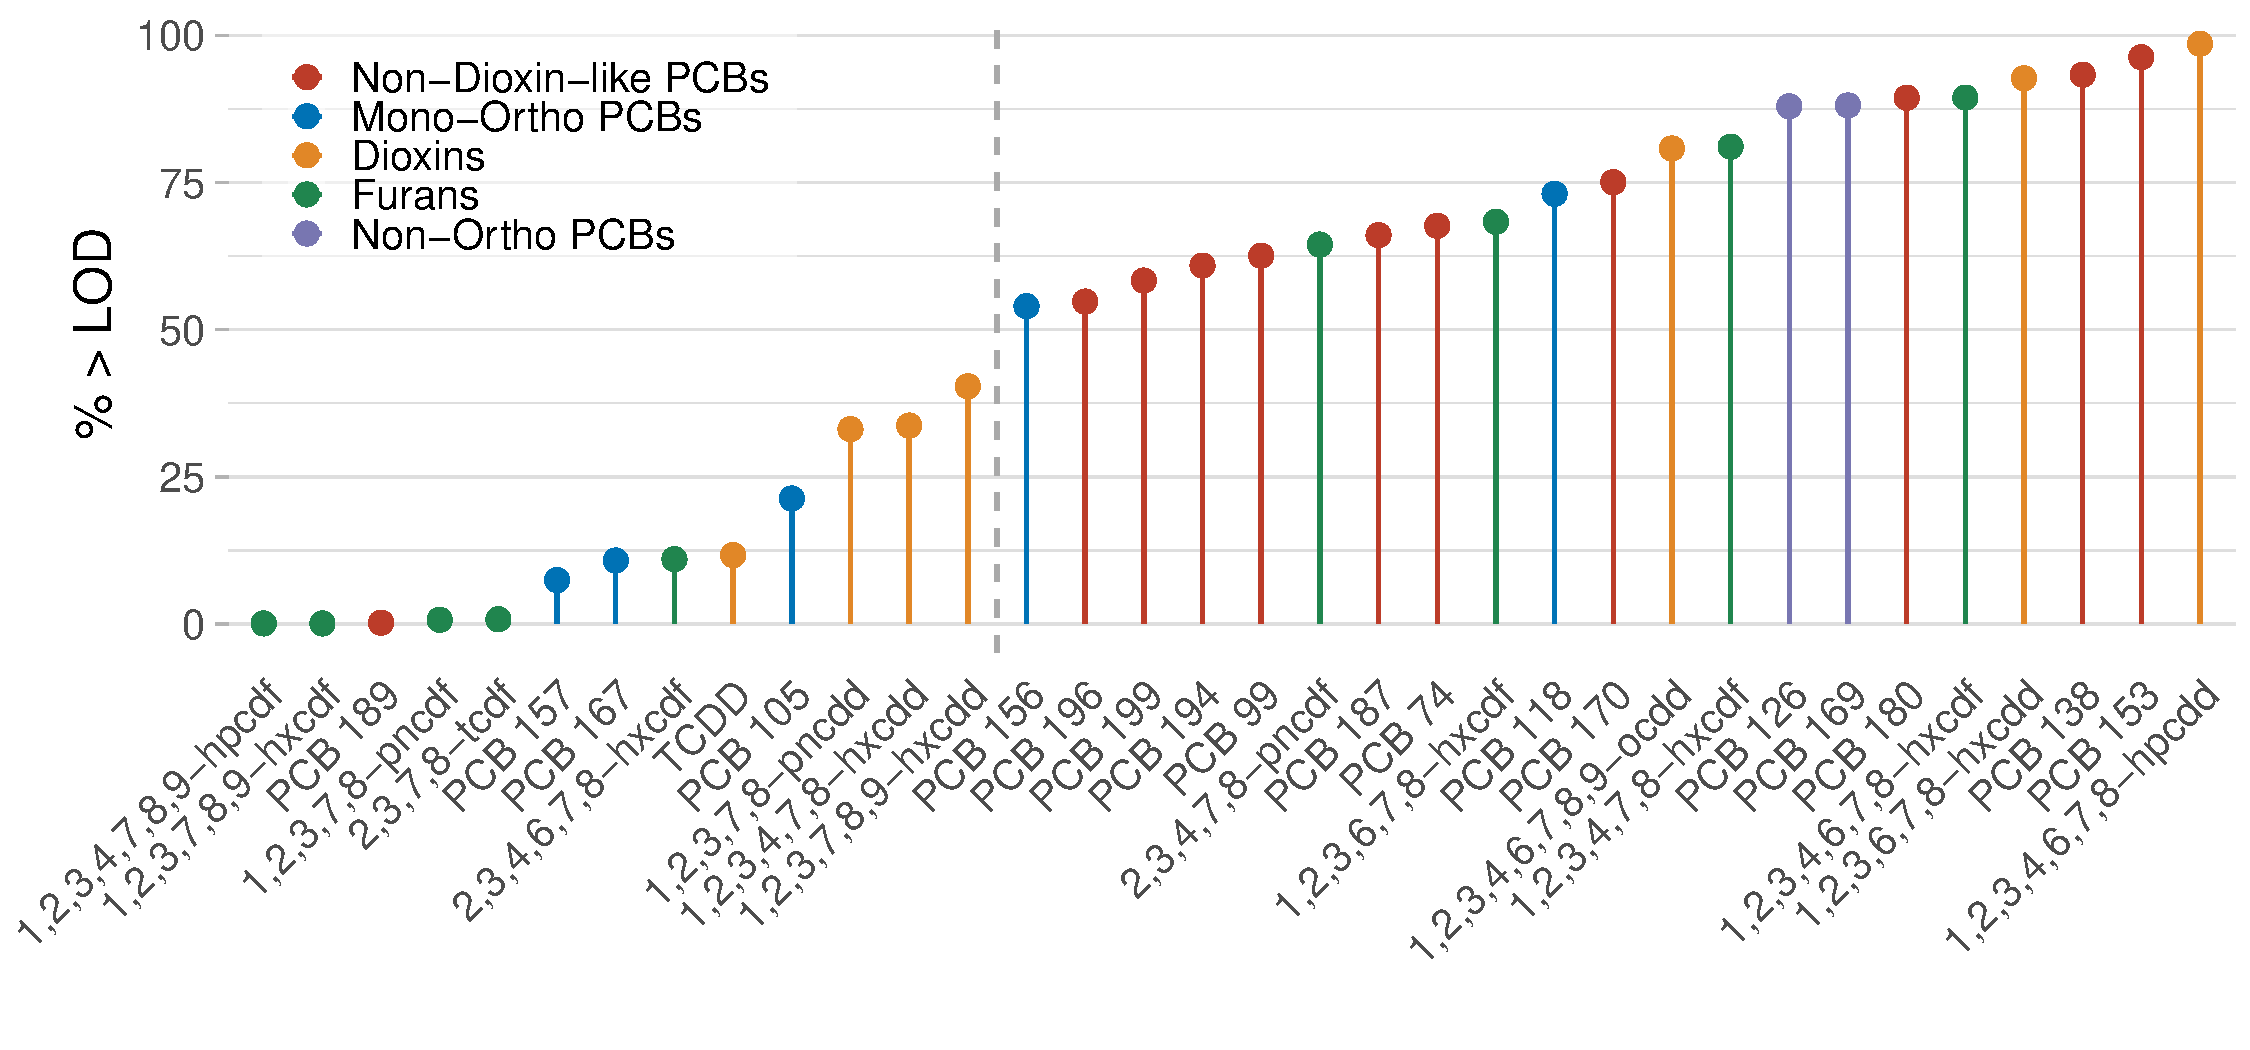
\includegraphics[scale=0.28]{figures/pcp/pop_detect.pdf}
\end{center}
}

\frame{\frametitle{PCP-LOD application: POP correlation}
\vspace{-1em}
\begin{center}
	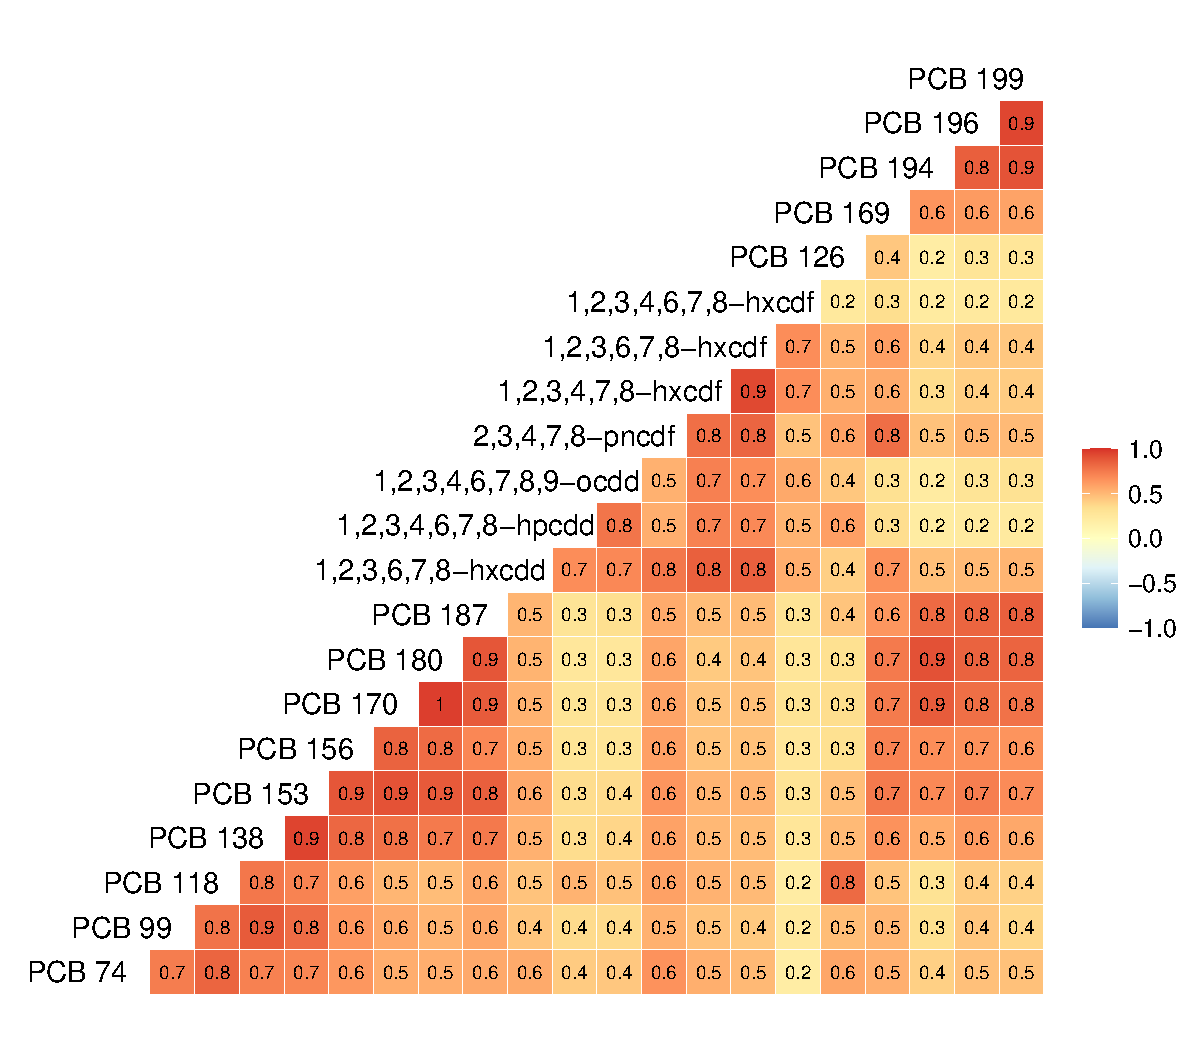
\includegraphics[scale=0.425]{figures/pcp/nhanes_raw_corr.pdf}
\end{center}
}

% low rank
\frame{\frametitle{NHANES results: 3 underlying patterns of POP exposure}
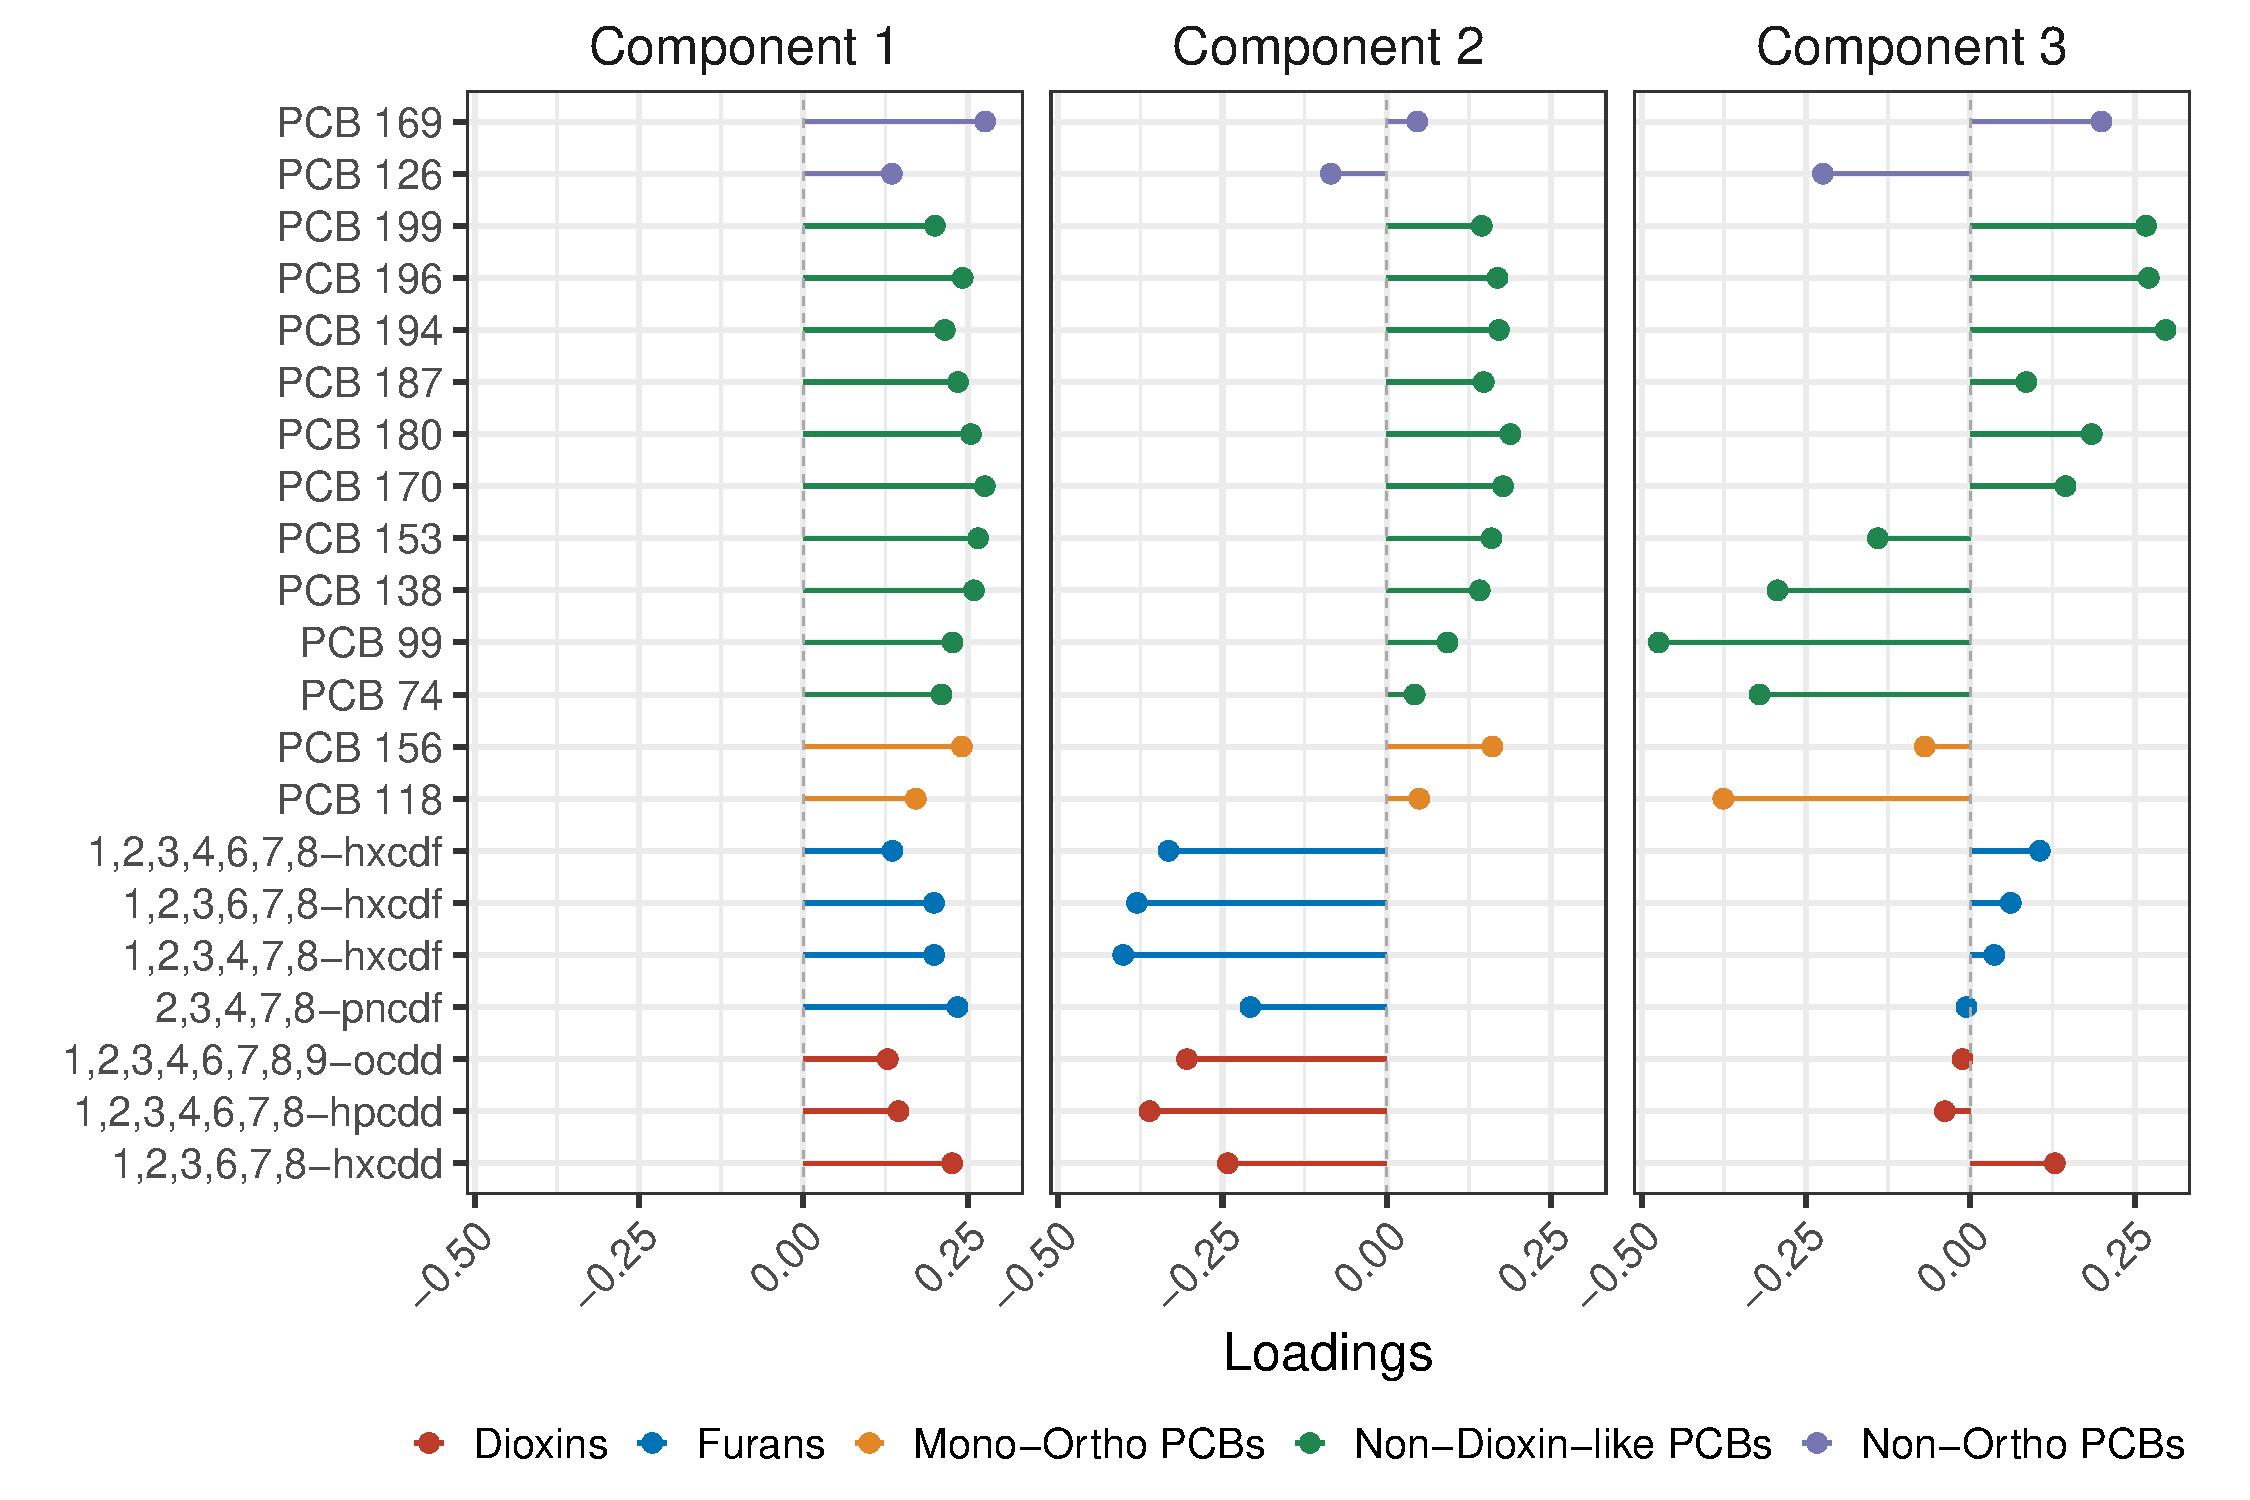
\includegraphics[scale=0.28]{figures/pcp/loadings.pdf}
}

% sparse
\frame{\frametitle{NHANES results: Sparse events not explained by patterns}
\vspace{-1.25ex}
\begin{center}
	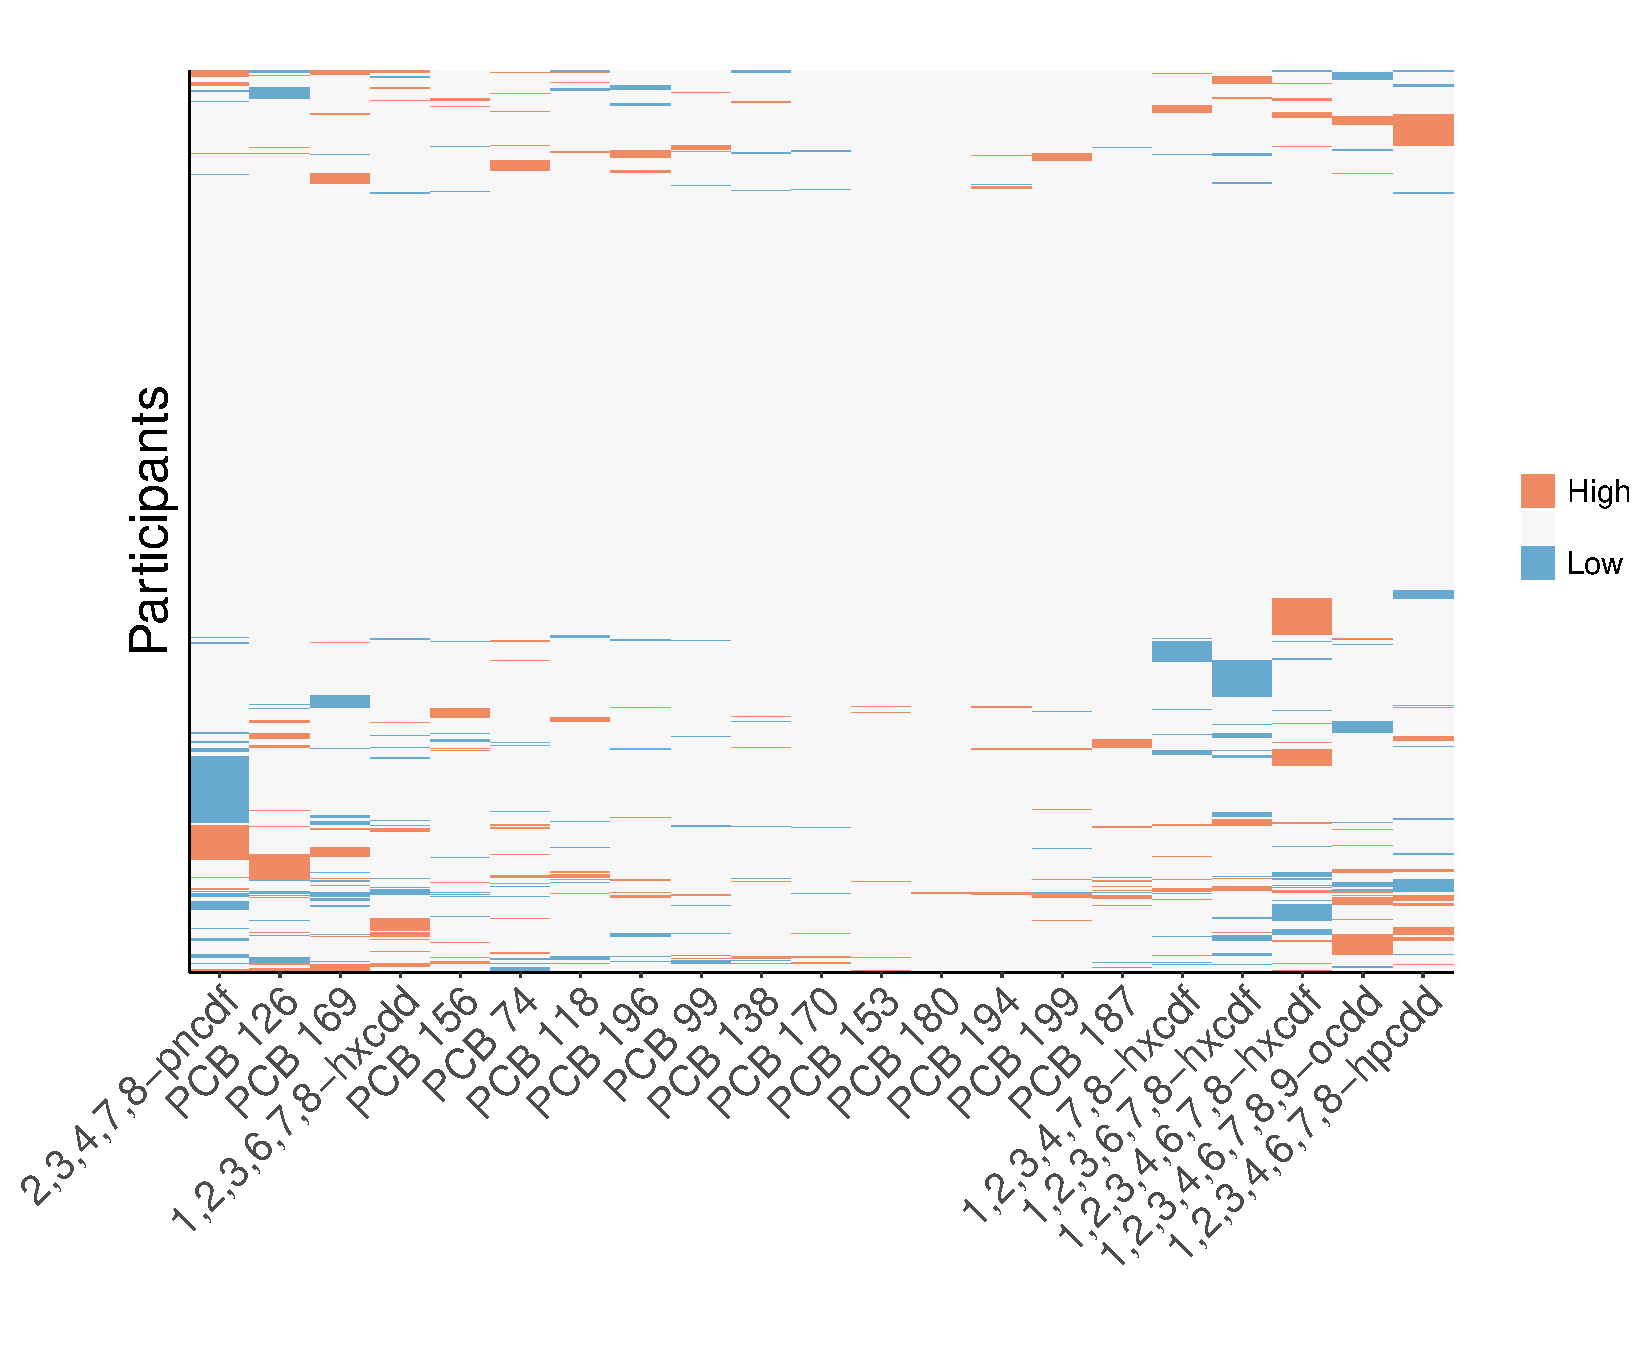
\includegraphics[scale=0.32]{figures/pcp/sparse_events.pdf}
\end{center}
}

\frame{
\frametitle{Principal component pursuit}
\begin{columns}[b]
\column{.6\textwidth}
\ \\
\vspace{2em}
\centering\color{matbluedark}{\LARGE\texttt{\textbf{BIG PICTURE}}}
\vspace{.5\baselineskip}
\begin{itemize}
         \item Patterns not influenced by outliers
         \item Extreme events separated, \\ not discarded
         \item Novel $<$ LOD penalty
         \item Potential for enhanced interpretability
         \item No parameter tuning
        \end{itemize}
\column{.4\textwidth}
\ \\ 
\vspace{2em}
\includesvg[scale=0.35]{figures/robot-svgrepo-com.svg}
\end{columns}
}